\section{Background} \label{sec:background}

In this chapter, we explain the essential concepts used in this work. We start by introducing Deep Learning and its main aspects. Then, we present \aclp{cnn} and Autoencoders, two types of Deep Architectures used by the proposed method. Also, an explanation about \acl{mtl} and its variants are presented. Later, we detail methods to explain Deep Networks, like \acs{shap}, and for dimensionality reduction, like \acl{pca} and \acs{tsne}. Next, the metrics proposed to evaluate the proposed work are detailed. Finally, the \icao standard is described, as well the \fvcongoing competition and its protocol.

\subsection{Deep Learning}

\acf{ai} is a study field of Computer Science focused on simulating the human intelligence process through machines. It can include, for example, learning, reasoning, and self-correction. In the early days of AI, the first systems were heavily based on a set of rules previously provided by an expert from some subject area. Usually, large rule-based problems are intellectually harder for humans than for computers and, thus, machines could take advantage. Also, such systems were developed for small and restricted environments. For example, we can cite Deep Blue \citep{hsu2002behind}, a successful chess-playing system developed by IBM which defeated the world champion, Garry Kasparov, in 1997.

As the scale and amount of data increased over the years, traditional AI methods have been replaced by a more data-driven approach, called \acf{ml}. Instead of manually providing rules for the system, an algorithm automatically learns the intrinsic patterns based on data. When desired answers are also provided as inputs, we call it \textit{Supervised Learning}; otherwise, it is called \textit{Unsupervised Learning}. Many algorithms have been developed for both types of learning, for instance: Support Vector Machines \citep{boser1992training}, Decision Trees \citep{breiman1984classification}, and Mean Shift \citep{fukunaga1975estimation}. 

Although \acl{ml} represented an important advance in the \acs{ai} field, traditional algorithms were limited when processing raw data in their natural form (for example, image pixels, text, or audio data). Typically, domain expertise was employed to carefully define how to extract useful features from raw data that could be used as inputs to the \acs{ml} algorithm. Such a process is usually called feature engineering. However, for many tasks, it may be difficult to define ``which'' and ``how'' features should be extracted (for instance, the features for detecting people in images).

Representation learning allows \acs{ml}-based systems to automatically discover valuable representations from raw data. According to \cite{goodfellow2016deep}, these learned representations often yield better performance in comparison to the hand-designed ones. Furthermore, representation learning algorithms also enable \acs{ai} systems a faster adaptation to new tasks with minimal human intervention.

% For instance, suppose we want to develop a \acs{ml}-based system to classify images from dogs, cats, and birds. As humans, we know that dogs usually have bigger snouts, cats have a mustache, and a bird has wings. However, describing these features in terms of image pixels can be a challenging task. Moreover, 

\acf{dl} represents a particular sub-field of representation learning which allows computational models composed of multiple processing layers capable of learning data representations with many levels of abstraction \citep{lecun2015deep}. Therefore, complex representations can be obtained by the composition of simpler ones. For example, we can cite the problem of detecting faces in images. The task of mathematically defining a function that maps a set of pixels (raw format) to the desired output (face location) can be very challenging. However, Deep Learning can solve this problem by breaking this complex mapping into a series of simple nested mappings, each described by a different model layer. For instance, the first layer may be responsible for detecting edges on raw pixels. Given these descriptions of edges, the second layer may look for corners and contours since they are defined by a set of edges. Consecutively, the third layer can detect entire object parts (e.g., eyes, nose, and mouth) by finding patterns in specific corners and contours. Finally, the parts of the object contained in the image can be evaluated to recognize the object's presence (or absence) in the image.

The most well-known examples of Deep Learning models are the \textbf{feedforward neural networks}, also called deep feedforward networks or multilayer perceptrons. They are inspired by the biological model of neurons, their connections, and how the human brain process information. The quintessential unit of a feedforward neural network is a node (neuron) that receives the inputs of other nodes and computes an output. Each input is associated with a learnable parameter $w$ (synapse), also called \textbf{weight}, that assigns relative importance to the correspondent input. The weighted sum of weights and inputs plus a \textbf{bias} compose the output of a neuron that is generally modified by an \textbf{activation function} responsible for introducing non-linearity to the network. A stack of nodes at the same level forms a layer, and sequences of layers compose the entire neural network. Each layer between the input and the output layer is called \textbf{hidden layer}. In a feedforward network, there are no feedback connections between the layers.

The set of weights and biases represents the trainable parameters of neural networks. Nevertheless, as with other \acs{ml} algorithms, the neural networks have other kinds of parameters, called \textbf{hyperparameters}. They are used to control the learning process and are commonly divided into two groups:

\begin{itemize}
\item \textbf{Model hyperparameters}: define aspects mainly related to the neural network architecture. For instance, we can cite the number of layers, the amount of neurons em each layer, the activation function of each layer, momentum, dropout rate, and others.

\item \textbf{Training hyperparameters}: related to the learning process itself. For example, the cost function, the number of epochs, optimizer, batch size, and many others.
\end{itemize}

It is crucial to notice that no optimal set of hyperparams can work for all kinds of particular problems, and their tuning is commonly performed manually. Also, while some hyperparams influence the time-and-memory cost to perform a prediction with the trained network, others affect the quality of the model and their capacity to output correct results when the network is presented to new inputs.

The rest of this section focuses on some specific kinds of neural networks and layers adopted in this work. Moreover, we describe a special kind of learning employed when networks may learn multiples tasks at the same time, called \acl{mtl}. Finally, we finish this section describing \acs{shap}, a state-of-art method to explain \aclp{dnn}.

\subsubsection{Convolutional Neural Networks}

\acfp{cnn}, also known as Convolutional Networks, are a specific kind of feedforward neural network specially developed to process grid-like data. For example, we can think of time-series data as a 1--D grid of time intervals with samples. Likewise, images can be considered as 2--D grid of pixels. In the last years, \acsp{cnn} have achieved exceptional performance in many practical applications. It includes, but it is not limited to, image classification \citep{li2014medical, guo2017simple, paoletti2018new}, object detection \citep{cai2016unified, wu2017squeezedet}, and instance segmentation \citep{wang2020solov2, xu2020convolutional, zhang2020mask}.

The convolution is the basic operation of a \acs{cnn}. In summary, it is a well-known mathematical operation that performs a linear calculation over two functions \citep{goodfellow2016deep}. It is similar to the cross-correlation, but one of the functions is reversed and shifted. Given the functions $x$ and $w$, the convolution operation between $x$ and $w$ - denoted by $h(t)$ - can be defined as in \autoref{eq:convolution}:

\begin{equation}
\label{eq:convolution}
h(t) = \int_{-\infty }^{\infty} x(\tau)w(t - \tau)\ d\tau
\end{equation}

\noindent
Typically, the convolution operation is expressed by an asterisk (\autoref{eq:conv_ast}):

\begin{equation}
\label{eq:conv_ast}
h(t) = (x * w)(t)
\end{equation}

\noindent
where $x$ represent the input, $w$ is the kernel, and $t$ is the moment where the convolution is computed. If $w$ is a valid probability density function, the convolution can be considered as a weighted average of the input at the moment $t$. Also, when working with discretized data (like digital images), the \autoref{eq:convolution} can be rewritten as \autoref{eq:conv_discrete}:

\begin{equation}
\label{eq:conv_discrete}
h(t) = \sum_{a=-\infty}^{\infty} x(\tau)w(t - \tau)
\end{equation}

Usually, \acsp{cnn} are primarily applied to process images as input. In these cases, the input $x$ is represented by 4--D vectors, also called tensors, of $N \times H \times W \times C$ dimensions, where $N$ denotes the number of images in the dataset (samples), $H$ and $W$ are the image dimensions, and $C$ corresponds to the number of channels of each image. The kernel $w$ is also a multidimensional array representing the parameters to be learned by the algorithm.

As pointed by \cite{goodfellow2016deep}, the convolution has three essential characteristics that help to improve the performance of ML-based systems:

\begin{itemize}
\item \textbf{sparse interactions}: in contrast to dense neural networks, the output units do not need to interact with each input unit. Instead, the kernel $w$ is commonly smaller than the input. Therefore, fewer parameters have to be stored, reducing the amount of memory required by the model, the number of operations and improving its statistical efficiency.

\item \textbf{parameter sharing}: refers to the reuse of the same kernel across the whole image. In traditional neural nets, each weight is applied strictly only once to compute the output of a layer. However, in \acsp{cnn}, the weights presented in the kernel $w$ are applied in every image pixel (except, in some cases, for the boundary pixels). Therefore, convolutions are dramatically more effective than dense matrix multiplications.

\item \textbf{equivariant representations}: refers to the fact that convolutions are invariant to translations. A function is called equivariant when the output changes correspond to the changes in the input. In mathematical terms, it means that a function $f(x)$ is equivariant to the function $g$ if $f(g(x)) = g(f(x))$. In the case of convolutions, if $g$ is a function that shifts the input image, the output of the convolution will be translated by the same amount. This property is useful to detect specific patterns across the image, like edges or even more complex shapes like faces. However, convolutions are not equivariant to transformations like image scaling or rotation.
\end{itemize}

In \aclp{cnn}, beyond the convolutional layers, there are also other common types of layers employed to perform other kinds of operations. Some other layers used in this work are described in the following subsections.

\paragraph{Pooling Layers}

Besides convolution, the pooling layers are one of the essential components of \aclp{cnn}. Pooling is an operation that provides an approach to reduce the spatial size of feature maps, also called downsampling, and summarize the features present in patches of the feature map. It helps to: (i) reduce the number of parameters; (ii) the number of computations performed in the network; and (iii) make the model more robust to slight variations in the position of features in the input image, controlling overfitting. In general, the pooling layers are applied after the activation function of convolutional layers and operates on each feature map independently.

There are two common types of pooling methods: \textbf{max pooling} and \textbf{average pooling}. They compute the maximum and the average value for each patch of the feature map, respectively. An example of both operations can be seen in \autoref{fig:poolings}.

\begin{figure*}[ht]
\centering
\subfigure[Max Pooling]{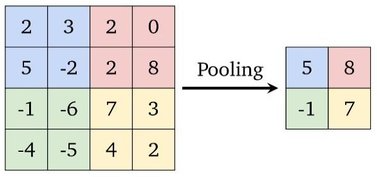
\includegraphics[width=0.4\linewidth]{images/pool_max.png}}
\hfill
\subfigure[Average Pooling]{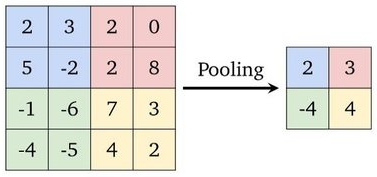
\includegraphics[width=0.4\linewidth]{images/pool_avg.png}}    
\caption{Example of Max Pooling and Average Pooling operations performed over a feature map of $4 \times 4$ with $pool\_size=2 \times 2$, $stride=2$, and no padding. Adapted from \citep{guissousallaeddine2019}.}
\label{fig:poolings}
\end{figure*}

The pooling layer has three input parameters: the filter size (also called pool size), the stride, and whether to apply padding to the input image. Commonly, the filter size is $2 \times 2$, the stride is 2, and no padding is applied. Using this configuration, the feature map is reduced by half at each dimension, and 75\% of the original activations are discarded. The number of channels of the feature map (depth) remains unchanged.

There is a special kind of pooling known as \textbf{global pooling}, introduced by \cite{lin2013network}. In addition to the traditional method, the global version extends the pooling across the entire feature map. Therefore, if a given feature map has $H \times W \times C$ dimensions, it will be reduced to $1 \times 1 \times C$. Again, the most common functions used in global pooling are maximum and average. As stated by \cite{zhou2016learning}, such difference makes global pooling layers perform better in practice than the conventional approach. Moreover, it can substitute the flattened layers in the transition between convolutional layers and the fully connected network responsible for outputting a prediction.

Since pooling computes a fixed function of the input, no learning parameters are required by the pooling layers in Convolutional Networks. This is valid for all pooling approaches described above (max, average, and global pooling).

\paragraph{Batch Normalization Layers}

The task of training deep neural networks can be challenging due to many factors. For example, we can cite the random weights initialization, the optimization algorithm, and the chosen hyperparameters configuration. Furthermore, during the learning phase, each parameter is updated by the gradient under the assumption that the other layers do not change \citep{goodfellow2016deep}. However, in practice, all layers are updated simultaneously.

Another significant factor is related to the expectations around layer distributions. During training, the distribution of each layer's input changes as previous layers' parameters also change. This is referred to as Internal Covariate Shift \citep{ioffe2015batch}. It may cause unintended effects in the training of deep networks since small changes in shallower layers will be amplified during a forward pass to deeper hidden layers.

Batch Normalization is a regularization technique proposed by \cite{ioffe2015batch} to mitigate the effect of Internal Covariate Shift. It normalizes the inputs of hidden layers using the first (mean) and second (variance) statistical moments of the current batch. This normalization step is usually applied before the activation function but can also be employed after the non-linear function. The batch normalization makes the training of deep neural networks faster, more stable, and less likely to overfit. Also, the batch normalization may substitute the use of Dropout as a regularization technique.

Given a mini-batch $B$ of size $m$, the mean and variance of $B$ are denoted by Equations \ref{eq:bn_mean} and \ref{eq:bn_stddev}, respectively:

\begin{equation}
\label{eq:bn_mean}
\mu_B = \frac{1}{m} \sum_{i}^{m} x_i
\end{equation}

\begin{equation}
\label{eq:bn_stddev}
\sigma_B^2 = \frac{1}{m} \sum_{i=1}^{m} (x_i - \mu_B)^{2}
\end{equation}

Then, the input $x_i$ is normalized by \autoref{eq:bn_norm}:

\begin{equation}
\label{eq:bn_norm}
\hat{x}_i = \frac{x_i - \mu_B}{\sqrt{\sigma_B^{2} + \epsilon}}
\end{equation}

\noindent
where $x_i$ can be either the input or output of the activation function from the current layer, and $\epsilon$ is a arbitrarily small constant added for numerical stability. The final output $y_i$ of the current layers is given by \autoref{eq:bn_output}:

\begin{equation}
\label{eq:bn_output}
y_i = \gamma\hat{x}_i + \beta
\end{equation}

\noindent
where $\gamma$ and $\beta$ are new learnable parameters introduced by batch normalization. 

One important aspect to notice is the fact that the batch normalization operation is reversible by itself. I.e., if the network during training realizes that the input $x_i$ does not need to be normalized, it can set $\gamma=1$ and $\beta=0$, so the input $x_i$ remains unchanged.

During the training phase, the normalization steps are computed based on mini-batches to ensure reliable and efficient training. On the other hand, during inference, the network is generally asked to perform prediction given a single sample. For this reason, the normalization step is performed with the population statistics estimated. The population mean and variance are estimated during training and are defined by Equations \ref{eq:bn_pop_mean} and \ref{eq:bn_pop_var}, respectively: 

\begin{equation}
\label{eq:bn_pop_mean}
E[x] = E_B[\mu_B]
\end{equation}

\begin{equation}
\label{eq:bn_pop_var}
Var[x] = \frac{m}{m-1} E_B[\sigma_B^{2}]
\end{equation}

Therefore, during inference, the input $x_i$ will be normalized by \autoref{eq:bn_inf_xi}:

\begin{equation}
\label{eq:bn_inf_xi}
\hat{x} = \frac{x_i - E[x]}{\sqrt{Var[x] + \epsilon}}
\end{equation}

And the output $y$ will be given by \autoref{eq:bn_inf_yi}:

\begin{equation}
\label{eq:bn_inf_yi}
y = \frac{\gamma}{\sqrt{Var[x] + \epsilon}} \cdot \hat{x} + \left( \beta - \frac{\gamma E[x]}{\sqrt{Var[x] + e}} \right)
\end{equation}

The implementation of batch normalization for \aclp{cnn} is slightly different in comparison to the fully connected networks. Since the output of \acs{cnn} layers can have multiple channels, batch normalization is carried out for each of these channels. In other words, each channel will have a single mean and standard deviation as well scale ($\gamma$) and shift ($\beta$) parameters. Again, they are scalar values learned during the optimization process. Similarly, the batch normalization procedure can be applied before or after the non-linear activation function of the correspondent convolutional layer.

Besides reducing the internal covariate shift, batch normalization also has some other valuable advantages. Firstly, it can speed up training since we can use higher learning rates without vanishing or exploding the gradients. Secondly, it can make the network more robust to different initialization schemes and learning rates. Finally, since batch normalization is a regularization technique, it helps the network improve in terms of generalization and diminish overfitting. As pointed out earlier, batch normalization can replace other regularization methods like Dropout.

Although the effect of batch normalization is evident, the explanation of why it works is still an open question. For example, some authors have suggested that the batch normalization does not reduce the internal covariance shift but actually smooths the objective function \citep{santurkar2018does}. Notwithstanding, batch normalization leads to harsh gradient explosion in deep networks at initialization, but such effect is mitigated by skip connections like the ones in residual networks \citep{yang2019mean}. Other authors suggest that the training of neural networks is faster with batch normalization due to the length-direction decoupling achieved by this technique \citep{kohler2019exponential}.

\subsubsection{Autoencoders}

Autoencoders represent a specific type of neural network capable of discovering structure within data to create a compressed representation of the input. They are considered an unsupervised (or self-supervised) learning technique to leverage the neural networks for representation learning. In the last years, Autoencoders have been successfully applied to many different tasks like: dimensionality reduction \citep{petscharnig2017dimensionality, wang2015dimensionality}, information retrieval tasks \citep{pfeiffer2018neural}, anomaly detection \citep{sakurada2014anomaly}, and image segmentation \citep{baur2018deep, karimpouli2019segmentation}.

The architecture of Autoencoders (\autoref{fig:autoencoder}) is usually composed of two parts:

\begin{figure}[h]
\centering
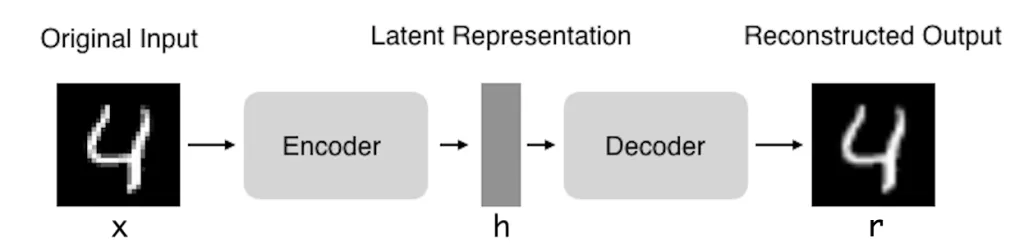
\includegraphics[width=\linewidth]{images/autoencoder.png}
\caption{Architecture of an Autoencoder. Source: \citep{autoencoder_architecture}}
\label{fig:autoencoder}
\end{figure}

\begin{enumerate}
\item \textbf{Encoder}: responsible to learn an useful representation of the input, also called \textbf{embeddings} or \textbf{latent representation} or even \textbf{code}. It can be formulated as an encoder function $h = f(x)$, where $x$ is the input and $h$ corresponds to the codification of the input in the latent space ($h: \mathbb{R}^D \rightarrow \mathbb{R}^K$)

\item \textbf{Decoder}: maps the learned latent representation $h$ back to the original input space ($\mathbb{R}^K \rightarrow \mathbb{R}^D$). It can be described as a reconstruction function $r = g(h)$, where $r$ is the reconstructed input.
\end{enumerate}

Since the exact copy of the input, $g(f(x)) = x$, is not especially useful, Autoencoders are intentionally designed to be unable to learn a perfect copy. Usually, Autoencoders are regularized in ways that allow them to learn an approximation of the identity function. By forcing the model to prioritize which input elements are relevant for reconstruction,  it often learns valuable properties of the data.

One typical Autoencoder architecture restricts the embedding dimensions ($h$) to be smaller than the input $x$. Such Autoencoder is called \textbf{undercomplete}. By constraining $h$, the Autoencoder is forced to learn an undercomplete representation and must prioritize the most salient features of the input data during training. Moreover, the reconstructed input $r$ will not be a perfect copy of the input, and the undercomplete Autoencoders can be considered lossy compressors.

The learning process of Autoencoders involves the minimization of a loss function like \autoref{eq:loss-basic}:

\begin{equation}
\label{eq:loss-basic}
L(x, g(f(x)))
\end{equation}

\noindent
where $L$ is a loss function that computes the similarity between the reconstructed input $g(f(x))$ and the original input $x$. For instance, $L$ can be the \acf{mse} or \acf{mae}

If the decoder is linear and $L$ is the \acs{mse}, the undercomplete Autoencoder will generate a subspace similar to PCA, described later in Section \ref{sec:pca} \citep{lecun2015deep}. On the other hand, Autoencoders with both non-linear encoder and decoder can learn a more powerful representation than PCA. However, if the encoder and decoder are too powerful, the Autoencoder can learn the identity function without extracting useful information about the data distribution. For instance, each training sample $x^{(i)}$ can be expressed as the code $i$, and the decoder can learn to map these integer indices back to the specific training examples. Nonetheless, it is rare to occur in practice \citep{lecun2015deep}.

Although the training of Autoencoders is similar to regular Neural Networks, some hyperparameters require special attention, like:

\begin{itemize}
\item \textbf{Embedding size}: the size of the latent representation represents a trade-off between compression and accurate reconstruction. Smaller size results in more compression, but the Autoencoder may be forced to drop relevant features for reconstruction. On the other hand, the higher the embedding size, the more likely is the Autoencoder to simply memorize or overfit the training data. Usually, this effect can be diminished by adding a term to the loss function that discourages memorization/overfitting (for instance, a regularizer).

\item \textbf{Number of Layers}: Vanilla Autoencoders are trained with a single hidden layer. However, training multilayer Autoencoders offers many advantages. First, depth can exponentially reduce the computation cost associated with representing some function. Furthermore, depth can also decrease the amount of training data needed to train a useful Autoencoder \citep{lecun2015deep}. Finally, experiments have shown that deep Autoencoders yield much better compression than equivalent shallow or linear Autoencoders \citep{hinton2006reducing}.

\item \textbf{Number of nodes per layer}: usually, Autoencoders have symmetric architecture. The number of nodes per layer in the encoder is the same as the decoder part but inverse. In the case of undercomplete Autoencoders, described earlier, the number of neurons per layer decreases at each layer and increases back in the decoder. In fact, symmetric architecture is not a mandatory rule but is commonly adopted in practice.

\item \textbf{Loss Function}: as discussed before, generally the \acs{mse} and \acs{mae} are used to measure the differences between the original input and the consequent reconstruction. Similarly, for the cases where the input is in the range [0-1], binary cross-entropy may also be used. However, other types of Autoencoders can apply different loss functions. For example, the Sparse Autoencoders adds a sparsity constraint (e.g., L1 regularization) as a penalty term such that only a fraction of the nodes will become active (i.e., nonzero values).
\end{itemize}

As pointed by \cite{lecun2015deep}, the lower-dimensional representations of Autoencoders have some benefits, like (i) it can improve the performance of tasks such as classification; (ii) fewer parameters require less memory and runtime; and (iii) the hints provided by the lower-dimensional space aid generalization.

\subsubsection{Multitask Learning}

\acf{mtl} is a recent machine learning technique in which multiple tasks are solved simultaneously, exploring common aspects and differences between them. This technique is inspired by the human learning process, where the knowledge obtained in previous problems is applied to learn the pattern of a new problem \citep{zhang2017survey}. Through \acs{mtl}, the network can use relevant information in related tasks to improve generalization in all tasks. Besides, this technique is best suited when there are limited training samples in multiple related tasks.

From the \acl{ml} point of view, \acl{mtl} can be seen as a form of inductive transfer. The goal of inductive transfer is to take advantage of additional information sources to increase the performance of the current task learning. It helps a model by introducing an inductive bias. Therefore, a model can prefer some hypotheses over others. A typical example of inductive bias is L1 regularization, which leads a model to prefer sparse solutions. In the context of \acs{mtl}, the inductive bias is supplied by the auxiliary tasks. In this case, the model will give preference to the hypothesis that explains more than one task. According to \cite{Caruana1997}, the inductive transfer can decrease the time of the learning process and increase the generalization and intelligibility of the model. 

Historically, \acs{mtl} methods were classified into hard or soft parameter sharing techniques \citep{vandenhende2021multi}. In the hard parameter sharing, initially proposed by \cite{Caruana1997}, the network parameters are divided into shared and task-specific parameters. Typically, \acs{mtl} models using hard parameter sharing contain a shared encoder with task-specific branches \citep{kendall2018multi, chen2018gradnorm, sener2018multi}. As proved by \cite{baxter1997bayesian}, the risk of overfitting in hard parameter sharing is order $N$ smaller than overfitting the task-specific branches, where $N$ is the number of tasks. Intuitively, since it is harder for a model to find a shared representation for all tasks, the less likely is the chance of overfitting. On the other hand, in soft parameter sharing, the parameters of each task are handled by a feature sharing mechanism \citep{ruder2019latent, gao2019nddr, liu2019end}. In this case, each task has a specific model, and the parameters of each model are regularized to be similar. \autoref{fig:mtl_sharing} visually explains the differences between hard and soft parameters sharing.

\begin{figure*}[ht]
\centering
\subfigure[Hard Parameter Sharing]{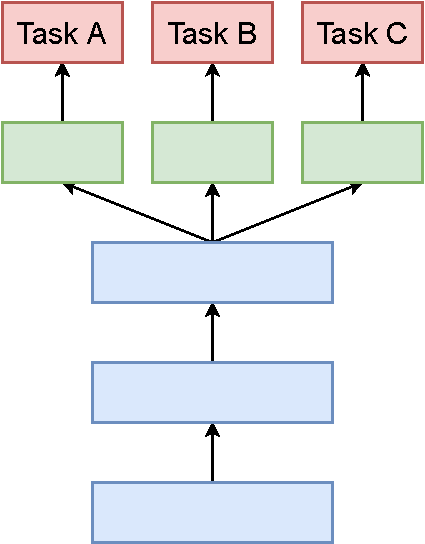
\includegraphics[height=0.35\linewidth]{images/mtl_hard.pdf}}
\hfill
\subfigure[Soft Parameter Sharing]{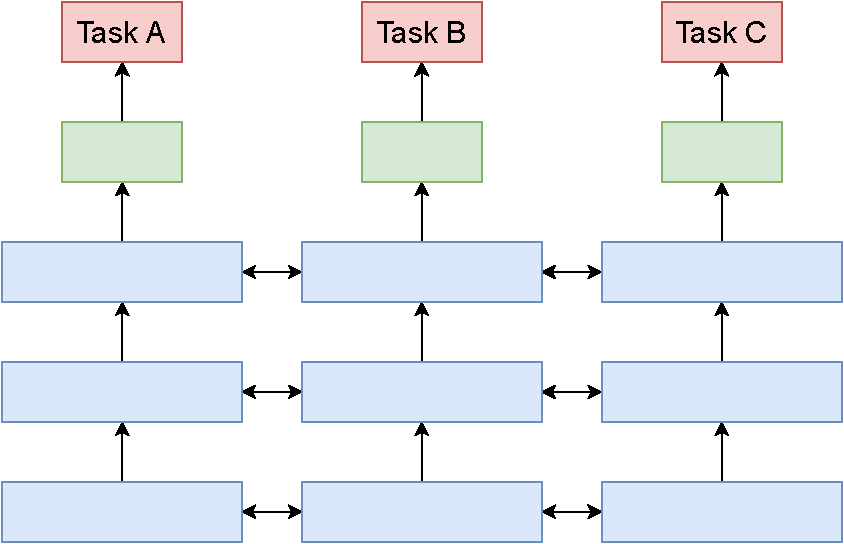
\includegraphics[height=0.35\linewidth]{images/mtl_soft.pdf}}    
\caption{Types of parameter sharing in \acl{mtl}. Source: own elaboration.}
\label{fig:mtl_sharing}
\end{figure*}

Compared to the case where each task of a multitask problem is solved individually by a specific network, the multitask networks present several advantages. First, the amount of parameters and memory used by the model is considerably reduced due to the inherent layer sharing. Secondly, the inference speed increases since such networks avoid the recomputation of features in the shared layers. Finally, such networks can improve performance if the related tasks share complementary information or act as a regularizer for one another \citep{vandenhende2021multi}. 

% In the context of the \icao standard, the MTL can be used to solve all requirements in parallel, reducing the processing time and increasing the success rates.

% \textbf{Multitask Optimization}. The optimization in MTL is still a significant challenge mainly because multiple learning procedures are being accomplished simultaneously. Therefore, one or more tasks can dominate the network weights or influence the gradients in opposite directions. To handle these problems, many approaches have been proposed in the literature over the years and will be discussed below.

% We can formulate the optimization of multitask problems without loss of generality as a function of task-specific weights $w_i$ and task-specific loss functions $\mathcal{L}$:

% \begin{equation}
% \label{eq:multitask-loss}
% \mathcal{L}_{MTL} = \sum_i {w_i \cdot \mathcal{L}_i}
% \end{equation}

% By using stochastic gradient descent to minimize the Eq. \ref{eq:multitask-loss}, the networks weights of a shared layer $W_sh$ are updated by the following rule:

% \begin{equation}
% \label{eq:multitask-sgd}
% W_{sh} = W_{sh} - \gamma \sum_i {w_i \frac{\partial \mathcal{L}_i}{\partial W_{sh}}}
% \end{equation}

\subsubsection{Network Explainability and Visualization}

For some time, the Deep Learning-based method was considered a black box since the interpretation of its outputs was hard to explain. To overcome this problem, some methods to visualize and explain predictions of Neural Networks have been proposed in the specialized literature. Some of the most well-known methods includes GradCam \citep{gradcam}, LIME \citep{lime}, DeepLIFT \citep{deeplift_old, deeplift_new}, and \acs{shap} \citep{shap2018}. In this section, we focus on detailing \acs{shap} since it is used to analyze the predictions of the proposed method. Furthermore, we cite other variations of \acs{shap} and highlight its advantages.

\paragraph{SHAP}

The \acf{shap} is a method to explain the output of any machine learning model using a solid theoretical foundation of game theory. The classic Shapley values \citep{shapley1953value} from game theory and their related extensions are combined to optimal credit allocation with local explanations. Nowadays, the method is considered the state-of-art method for \acs{ml} explainability.

The basic idea of \acs{shap} comes from the game theory. In summary, the Shapley values try to quantify the contribution that each player brings to a game. In the context of \acl{ml}, the ``game'' is considered as the outcome of the model, while the ``players'' are represented by one or more features included in the model. In the case of images, specifically, pixels can be grouped (superpixels) to explain predictions distributed among them. Therefore, the goal of SHAP is to measure the contribution of each feature concerning the model's prediction.

Given the original prediction model $f$ to be explained and the explanation model $g$, the Shapley value explanation is represented as an additive feature attribution method (\autoref{eq:shap_add}), which is a linear function of binary values:

\begin{equation}
\label{eq:shap_add}
g(z')=\phi_0+\sum_{j=1}^M\phi_jz_j'
\end{equation}

\noindent
where $z' \in \{0,1\}^M$ is the coalition (subset) vector, $M$ is the number of simplified input features (coalition size) and $\phi \in \mathbb{R}$ is the feature attribution for a feature $j$ (Shapley values). Many methods has explanation models that matches the \autoref{eq:shap_add}, including \acs{lime} \citep{lime} and \textit{DeepLIFT} \citep{deeplift_old, deeplift_new}.

To compute the contribution of each feature ($\phi_i$), the \acs{shap} method requires retraining the model on all subset of features $S \subseteq F$, being $F$ the full set of features. A corresponding importance value will be assigned to each feature to represent the effect on the model prediction when such feature is included. To compute this effect, a model is trained with the presence of that feature ($f_{S \cup \{i\}}$), and another model is trained without that feature ($f_S$). Then, the predictions of the two models are compared for the current input $f_{S \cup \{i\}}(x_{S \cup \{i\}}) - f_S(x_S)$. In this case, $x_S$ denotes the values of the input features in the set $S$. The preceding differences are computed for all possible subsets since the effect of withholding a feature also depends of other features in the model. The Shapley values are the weighted average of all possible differences (\autoref{eq:shapley-values}):

\begin{equation}
\label{eq:shapley-values}
\phi_i = \sum_{S \subseteq F \setminus \{i\}} \frac{\left|S\right|!(\left|F\right| - \left|S\right| - 1)!}{\left|F\right|!}\left[f_{S \cup \{i\}}\right (x_{S \cup \{i\}}) - f_S(x_S)]
\end{equation}

Since a model is trained for every subset of $S$, the exact computation of Shapley values is computationally expensive. For $F$ features, there is a total of $2^F$ subsets of S. However, in the paper of \acs{shap} \citep{shap2018}, the authors propose a model-agnostic approach to approximate them, called Kernel SHAP, and other four model-type-specific approximation methods: Linear SHAP, Low-Order SHAP, Max SHAP, and Deep SHAP. The Deep SHAP is a specific version of \acs{shap} especially designed for Deep Networks. The method is based on DeepLift \citep{deeplift_old, deeplift_new}, which approximates SHAP values by considering the input features as independent of each other and the deep model as linear. In Deep SHAP, the SHAP values of the whole network are a combination of SHAP values computed for smaller components of the network. It generates an effective linearization from the SHAP values computed for each component. Please, refer to the original paper for further explanations on the other methods.

The SHAP method has the four properties of classical Shapley values:

\begin{enumerate}
\item \textbf{Efficiency:} the sum of the Shapley values for all players is equal to the value of the total coalition. 
\item \textbf{Symmetry}: all players have a fair chance to join the game.
\item \textbf{Dummy}: if a player $i$ has no contribution to a coalition $S$ (i.e., for each $S$, $f_{S \cup \{i\}} = f_S$), then its contributions is zero ($\phi_i = 0$).
\item \textbf{Additivity}: for any pair of games $a$ and $b$, $\phi(a + b) = \phi(a) + \phi(b)$. Such property enables simple arithmetic summations.
\end{enumerate}

Some of the main advantages of \acs{shap} are discussed next. First, it is model agnostic, i.e., \acs{shap} makes no prior assumption of the model and can work with any \acs{ml} algorithm. Secondly, the method ensures consistency. It means that even if features are removed from data, the others keep contributing with the same importance (Shapley values). Lastly, \acs{shap} can explain not only how each feature contributes regarding each sample (\textit{local interpretability}), but also at a global level (\textit{global interpretability}) by aggregating the local results.

\subsection{Dimensionality Reduction}

There are many applications for algorithms of dimensionality reduction. Usually, these methods are used when the cardinality of features is significantly larger than the number of samples (also called the ``\textit{curse of dimensionality}''). However, they may also be applied to project data into a lower-dimensional space (usually 2D/3D), aiming to simplify visualization and the search for patterns in data. In this subsection, two methods of dimensionality reductions used in this work are described.

\subsubsection{Principal Component Analysis}
\label{sec:pca}

The \acf{pca} \citep{pca} is an unsupervised \acl{ml} algorithm for dimensionality reduction with minimal information loss. In PCA, the information is based on the data variance. The idea is that features with high variance contain more information because their data are more distributed than features with low variance. Accordingly, the PCA projects the data into a subspace where the axis with the highest variances, also called \textit{principal components}, are preserved. More details of PCA are described below.

The main step of PCA is to compute the \textbf{eigenvectors} (principal components) of the input data. The eigenvectors explain the variance of data along the new axes and determine the direction in the new feature space. In PCA, they are organized into a projection matrix, and each eigenvector is associated with an \textbf{eigenvalue}. The eigenvalue can be interpreted as the magnitude of the corresponding eigenvector. If the eigenvalues have a similar magnitude, it can be considered a valuable indicator that the original data is already in a suitable subspace. Otherwise, if the magnitude of some eigenvalues is much higher than others, the corresponding eigenvectors may be chosen since they contain more information about our data distribution. Likewise, the eigenvalues near zero are less informative and may be discarded in the construction of the new subspace. 

The classical approach of PCA \citep{pca} computes the covariance matrix, where each element represents the covariance between two features, computed by \autoref{eq:covariance}:

\begin{equation}
\label{eq:covariance}
\sigma_{jk} = \frac{1}{n-1}\sum_{i-1}^{N}(x_{ij} - \bar{x_j})(x_{ik} - \bar{x}_k)
\end{equation}

\noindent
which can be rewritten in the matrix form as \autoref{eq:covariance2}:

\begin{equation}
\label{eq:covariance2}
S = \frac{1}{n-1}((x - \bar{x})^T(x - \bar{x}))
\end{equation}

\noindent
where $\bar{x}$ is a D-dimensional vector in which each value corresponds to the average of each feature, and $n$ is the number of features per sample. Also, $x$ is the data matrix, where a row represents each sample, and the features are columns. In practice, if we have a dataset with four features, for instance, the covariance matrix will have the following structure:

$$
\begin{bmatrix}var(1) & cov(1,2) & cov(1,3) & cov(1,4) 
\\ cov(1,2) & var(2) & cov(2,3) & cov(2,4)
\\ cov(1,3) & cov(2,3) & var(3) & cov(3,4)
\\ cov(1,4) & cov(2,4) & cov(3,4) & var(4)
\end{bmatrix}
$$

\noindent
where the main diagonal corresponds to the variance of each dimension, and the remaining elements are the covariance between each dimension pair. An interesting property of the covariance matrix is that the sum of the main diagonal is always equal to the sum of eigenvalues.

The eigenvectors and eigenvalues of PCA can also be computed using the correlation matrix. Although the resulting matrices are different, they will result in the same eigenvectors and eigenvalues since the correlation matrix is given by the standardization of the covariance matrix (\autoref{eq:correlation}):

\begin{equation}
\label{eq:correlation}
corr(x,y) = \frac{cov(x,y)}{\sigma_x \sigma_y}
\end{equation}

Given the projection matrix $W$ computed by PCA, we can project our original data $X$ into the new subspace $S$ by applying the \autoref{eq:pca_transform}:

\begin{equation}
\label{eq:pca_transform}
S = (X-\mu_X) \times W
\end{equation}

\noindent
where $\mu_X$ represents the mean of each feature column in $X$.

Note that we can rollback to our original space $X$ by application of \autoref{eq:pca_inverse}:

\begin{equation}
\label{eq:pca_inverse}
X = (S \times W^{-1}) + \mu_X
\end{equation}

Finally, the \acf{lda} \citep{izenman2013linear} is a similar dimensionality reduction technique. In contrast to \acs{pca}, the \acs{lda} is a supervised method that maximizes the component axes for class-separation. Although it looks like \acs{lda} performs better than \acs{pca} in reducing dimensionality for classification problems, this is not always true. Performance comparison in terms of accuracy for image recognition problems has shown that \acs{pca} has performed better than \acs{lda} if the number of samples per class is relatively low \citep{martinez2001pca}.

\subsubsection{t-SNE}

The \acf{tsne}, developed by \cite{tsne}, is a non-linear method of dimensionality reduction that is particularly well suited for visualization of high-dimensional datasets. It is based on Stochastic Neighbor Embedding \citep{sne}, but the main difference is the utilization of the \textit{t}-Student distribution to represent the data in low dimensions.

The \acs{tsne} algorithm has two main stages. First, the symmetric probability of points in the original high-dimensional space is computed. Higher probabilities are assigned to similar points, while dissimilar points are assigned a lower probability. Such probabilities are computed using a \textit{t}-Student kernel with a given degree of freedom. Secondly, a similar probability distribution is defined over the points mapped into the low-dimensional space. The Kullback-Leibler divergence (also called relative entropy) between these two distributions is minimized through a gradient descent technique. A simplified version of \acs{tsne} is shown in Algorithm \ref{alg:tsne} and the details are explained below.

\begin{algorithm}[t]
\caption{Simple version of t-Distributed Stochastic Neighbor Embedding}
\label{alg:tsne}
\begin{algorithmic}
    \State \textbf{Data:} data set $X = \{x_1, x_2, ..., x_n\}$,
    \State cost function parameter: perplexity $Perp$,
    \State optimization parameters: number of iteration $T$, learning rate $\eta$, momentum $\alpha(t)$.
    \State \textbf{Result:} low-dimensional data representation $\gamma^{(T)} = \{y_1, y_2, ..., y_n\}$.
    \Begin 
        \State compute pairwise affinities $p_{j|i}$ with perplexity $Perp$ (using \autoref{eq:tsne_pij})
        \State set $p_{ij} = \frac{p_{j|i} + p_{i|j}}{2n}$
        \State sample initial solution $\gamma^{(0)} = \{y_1, y_2, ..., y_n\}$ from $\mathcal{N}(0, 10^{-4}I)$
        \For{i=1}{T}
        \Begin
            \State compute low-dimensional affinities $q_{ij}$ (using \autoref{eq:tsne_qij})
            \State compute gradient $\frac{\partial C}{\partial \gamma}$ (using \autoref{eq:tsne_grad})
            \State set $\gamma^{(t)} = \gamma^{(t-1)} + \eta \frac{\partial C}{\partial \gamma} + \alpha(t)(\gamma^{(t-1)} - \gamma^{(t-2)})$
        \End
    \End
\end{algorithmic}
\end{algorithm}

Given an object $i$, and each potential neighbor $j$ in the high-dimensional space, the joint probability $p_{ij}$ that computes the pairwise similarity between $i$ and $j$ is defined as in \autoref{eq:tsne_pij}:

\begin{equation}
\label{eq:tsne_pij}
p_{ij} = \frac{exp(-d_{ij}^2)}{\sum_{k \neq i}exp(-d_{ik}^2)}
\end{equation}

In the original SNE, a conditional probability $p_{i|j}$ is used instead. Also, the t-SNE employs the scaled Euclidean Distance as the dissimilarity metric $d_{ij}^2$ between two high-dimensional points $x_i$ and $x_j$ (\autoref{eq:tsne_dij}). However, other distance metrics can be used when appropriate. One important detail to notice is the fact that he pairwise similarity $p_{ij}$ is not robust to outliers since $\left\| x_i - x_j\right\|^2$ will be large. In theses cases, the values of $p_{ij}$ will be extremely small and the location of its low-dimensional map point will have very little effect over the cost function. In practice, such problem is prevented by computing $p_{ij} = \frac{p_{j|i} + p_{i|j}}{2n}$ instead. This ensures that $\sum_j p_{ij} > \frac{1}{2n}$ for all datapoints $x_i$. As a result, each datapoint $x_i$ has a significant higher contribution to the cost function.

\begin{equation}
\label{eq:tsne_dij}
d_{ij}^2 = \frac{\left\| x_i - x_j \right\|^2}{2\sigma_i^2}
\end{equation}

\noindent
where $\sigma_i$ can be either defined by hand or via a binary search that makes the entropy of the distribution over neighbors equal to $log\ Perp$. In this case, $Perp$ is an input parameter of the cost function called ``perplexity.'' The perplexity may be interpreted as a measure of the effective number of neighbors and is defined by \autoref{eq:tsne_perp}:

\begin{equation}
\label{eq:tsne_perp}
Perp(P_i) = 2^{H(P_i)}
\end{equation}

\noindent
where $H(P_i)$ is the Shannon entropy of probability $P_i$ measured in bits by \autoref{eq:tsne_entropy}:

\begin{equation}
\label{eq:tsne_entropy}
H(P_i) = -\sum_j p_{j|i}\ log_2\ p_{j|i}
\end{equation}

In general, the performance of t-SNE is reasonably robust to changes in perplexity, and typical values are between 5 and 50.

The similarity in the low-dimensional space is given by \autoref{eq:tsne_qij}:

\begin{equation}
\label{eq:tsne_qij}
q_{ij} = \frac{exp(-\left\| y_i - y_j \right\|^2)}{\sum_{k \neq i} exp(-\left\| y_i - y_k \right\|^2)}
\end{equation}

\noindent
where $y_i$ and $y_j$ represent the low-dimensional counterparts of the
high-dimensional data points $x_i$ and $x_j$. Usually, for tasks in which the dimensionality of the data is reduced to 2D or 3D, the \textit{t}-Student distribution is applied with one degree of freedom and the \autoref{eq:tsne_qij} can be rewritten as \autoref{eq:tsne_qij_1}:

\begin{equation}
\label{eq:tsne_qij_1}
q_{ij} = \frac{(1 +\left\| y_i - y_j \right\|^2)^{-1}}{\sum_{k \neq l} (1 +\left\| y_k - y_l \right\|^2)^{-1}}
\end{equation}

Finally, the \acs{tsne} tries to minimize a single Kullback-Leible divergence (\autoref{eq:tsne_cost}) between a joint probability distribution $P$ in the high-dimensional space and a joint probability distribution $Q$ in the low-dimensional space:

\begin{equation}
\label{eq:tsne_cost}
C = KL(P||Q) = \sum_i\sum_j p_{ij} log \frac{p_{ij}}{q_{ij}}
\end{equation}

In contrast to the SNE implementation, the \acs{tsne} is symmetric since $p_{ij} = p_{ji}$ and $q_{ij} = q_{ji}$ $\forall i,j$. The main advantage of such symmetry is the simpler gradient expression, being faster to compute. The gradient of the cost function $C$ with respect to the point $y_i$ is given by \autoref{eq:tsne_grad}:

\begin{equation}
\label{eq:tsne_grad}
\frac{\partial C}{\partial y_i} = 4 \sum_j (p_{ij} - q_{ij})(y_i - y_j)
\end{equation}

And the set $\gamma^{(t)} = \{y_1, y_2, ..., y_N\}$ will be updated by a momentum term given by \autoref{eq:tsne_update}:

\begin{equation}
\label{eq:tsne_update}
\gamma^{(t)} = \gamma^{(t-1)} + \eta\frac{\partial C}{\partial \gamma} + \alpha(t)(\gamma^{(t-1)} - \gamma^{(t-2)})
\end{equation}

\noindent
where $\gamma^{(t)}$ indicates the solution at iteration $t$, $\eta$ is the learning rate, and $\alpha(t)$ represents the momentum at iteration $t$. For derivation of \acs{tsne} gradient, please refer to Appendix A of \citep{tsne}. 

In comparison to \acs{pca}, the \acs{tsne} does not conserve the distances or the densities of the original space. Only the neighborhood is preserved, but up to a certain degree. Furthermore, there is no convergence guarantee to the global optimum of the cost function, and the performance of \acs{tsne} is not clearly defined for general dimensionality reduction tasks. 


\subsection{Performance Measures} \label{sec:measures}

There is a variety of performance measures to evaluate algorithms in binary classification problems. In common, most of these metrics takes into account some of/all the four possible results presents in the binary confusion matrix: \acfp{tp}, \acfp{tn}, \acfp{fp}, and \acfp{fn}. In this subsection, we describe the evaluation metrics used in this work. Comments about the advantages and disadvantages of each one are also made when appropriate. 

\subsubsection{Accuracy}

Accuracy is one of the most used metrics to evaluate binary classifiers. In simple terms, it measures how many predictions were correct among all samples in a given dataset. The output of this metric a score $\in [0, 1]$ which is interpreted as the proportion of correct predictions (i.e., true positives and true negatives) among the total number of samples analyzed. The Accuracy is described by the \autoref{eq:accuracy}:

\begin{equation}
\label{eq:accuracy}
Accuracy = \frac{TP + TN}{TP + TN + FP + FN}
\end{equation}

Although Accuracy is one of the most used metrics to evaluate binary classifiers, it is not well suited for unbalanced datasets. Suppose we have a dataset where 80\% of samples are from the positive class, and the remaining samples are from the negative class. If some classifier outputs only the positive class, the overall Accuracy will be 80\%. Therefore, Accuracy must only be considered a valid metric when the class distributions are considerably uniform.

\subsubsection{Precision \& Recall} \label{precision-recall}

Precision and Recall are two metrics highly adopted in the evaluation of binary classifiers. While Precision measures how much we can trust a model when it predicts the positive class, the Recall measures how accurate a model is regarding the positive class. In other words, the Precision metric answers the question ``\textit{given the positive predictions, how many were correct?}'', while Recall answers ``\textit{given the positive samples, how many predictions were correct?}''. Precision and Recall are also known as \acf{ppv} and Sensitivity, respectively, and they are defined by Equations \ref{eq:precision} and \ref{eq:recall}: 

\begin{equation}
\label{eq:precision}
Precision = \frac{TP}{TP + FP}
\end{equation}

\begin{equation}
\label{eq:recall}
Recall = \frac{TP}{TP + FN}
\end{equation}

Even though the Precision and Recall metrics are considered more robust than Accuracy to evaluate binary classifiers, both metrics present some drawbacks. First, they are purpose-specific. For example, Precision is a better choice when we want to trust the prediction of the positive class. However, if a model is optimized to maximize Precision only, it can bias the classifier to avoid uncertain positive samples, increasing the false negatives. On the other hand, Recall is more pertinent when we need a classifier that may correctly identify the positive samples, although it can generate more false positives. Hence, in case of a problem where Precision and Recall are equally important, the f-measure may be computed to generate a balanced score between these two metrics. The f-measure is better described in the following subsection.

Secondly, by taking a closer looker at the Equations \ref{eq:precision} and \ref{eq:recall}, we can notice that they do not take into account the True Negatives. Therefore, both metrics are more appropriate when the positive class is more important than the negative class. It is the case of detection problems, for example, where identifying the negative class (usually background) is less important than the positive class (object of interest). Nevertheless, for some classification problems, this is not always true. For instance, we can cite the fraud detection problems, where the correct prediction of the True Negatives has a higher priority over the True Positives. For these cases, we can compute the negative predictive value and specificity metrics, which are described later.

\subsubsection{F-measure}

The f-measure, also called f-score or f1-score, is a metric to balance the values of Precision and Recall. The importance of f-measure is better understood by an example. Suppose there is a face detection problem, where two different models are applied in an image with ten faces, named $A$ and $B$. Model A returned five detections, where 3 were real faces (TP), and 2 were incorrect. In this case, model A has 30\% of Recall (3 out of 10 detected faces) and 60\% of Precision (3 out of 5 correct predictions). Otherwise, model B returned two detections, and they are all real faces. In this case, the Recall is 20\% (2 out of 10 detected faces), and the Precision is 100\% (all detections are real faces). Therefore, if Precision and Recall are equally important for this problem, which model is better: model $A$ with 30\% of Recall and 60\% of Precision, or model $B$ with 20\% of Recall and 100\% of Precision? To answer this problem, we can compute the f-measure, described by \autoref{eq:f-measure}: 

\begin{equation}
\label{eq:f-measure}
F{-}Measure = 2\frac{Precision \cdot Recall}{Precision + Recall}
\end{equation}

In the example cited above, the f-measure of model $A$ is 40\%, while the model $B$ is 33.3\%. Therefore, the model $A$ can be considered a better model for this case since it has a higher f-measure and consequently a better equilibrium between Precision and Recall.

By definition, the f-measure is considered the harmonic mean between Precision and Recall. It is harmonic because, in contrast to the arithmetic mean, the metric cannot be made arbitrarily large by changing only Precision or Recall to a bigger value (while keeping the other metric unchanged). Therefore, to increase f-measure considerably, both Precision and Recall must be higher at the same time.

\subsubsection{F-Beta}

The F-Beta is a generalization of the F-measure. It adds a $\beta$ term to weight how much Recall is more important than Precision. The F-Beta is defined by \autoref{eq:f-beta}:

\begin{equation}
\label{eq:f-beta}
F_\beta = \frac{(1 + \beta^2) \cdot P \cdot R}{\beta^2 \cdot P + R}
\end{equation}

As can be noticed, when $\beta=1$, we have the original formula of f1-score. Another typical value is $\beta=2$, generating the f2-score. In this case, we are considering that Recall has a higher weight than precision. In other words, achieving a better Recall is more important for the classifier than Precision. It is useful when we want to make sure that the classifier is better at identifying the positive class, even though it might generate more false positives. In the detection example cited before, the detector would try to detect as many real faces as possible but probably returning more false positives (detections that are not real faces).

\subsubsection{Negative Predictive Value \& Specificity}

The metrics specificity and \acf{npv} are equivalent to Recall and Precision, respectively, but for the negative class. In analogy to Precision and Recall, the specificity answers the question ``\textit{given the negative samples, how many predictions were correct?}'', while the \acs{npv} answers ``\textit{given the negative predictions, how many were correct?}''. The metrics are defined by Equations \ref{eq:specificity} and \ref{eq:npv}:

\begin{equation}
\label{eq:specificity}
Specificity = \frac{TN}{TN + FP}
\end{equation}

\begin{equation}
\label{eq:npv}
NPV = \frac{TN}{TN + FN}
\end{equation}

Since both \acs{npv} and specificity are similar to Precision and Recall, they share the same problems of these metrics described in Section \ref{precision-recall}. Hence, \acs{npv} and specificity are purpose-specific (but, for the negative class) and, analogously, do not take into consideration the positive class.

\subsubsection{\acl{mcc}} \label{sec:mcc}

The \acf{mcc}, also known as phi coefficient, is a binary classification metric that takes into account all the four confusion matrix categories: true positives, true negatives, false positives, and false negatives. It was introduced by biochemist Brian W. Matthews in 1975 \citep{matthews1975comparison} and is defined by the \autoref{eq:mcc}

\begin{equation}
\label{eq:mcc}
MCC = \frac{TP \times TN - FP \times FN}{\sqrt{(TP + FP)(TP + FN)(TN + FP)(TN + FN)}}
\end{equation}

The \acs{mcc} is considered a balanced metric and can be used even in highly unbalanced datasets. The output of \acs{mcc} is normalized coefficient between $-1$ and $+1$. A coefficient of $+1$ means a perfect prediction, while $-1$ represents a total disagreement between prediction and ground truth. Also, a coefficient of $0$ represents that the predictions are no better than random guesses. 

Since the \acs{mcc} takes into account the four possible results of binary classification problems, it presents some advantages in comparison to other classification metrics. For example, given a trained classifier with a confusion matrix of TP = 90, \acs{fp} = 5, TN = 1, and FN = 4, in this case the Accuracy is 91\% and the f-measure is 95.24\%. On the other hand, the \acs{mcc} gives a score of 0.14, which means the algorithm is basically predicting the most frequent class and performing similarly to random guessing. As suggested by \cite{chicco2017ten}, the \acs{mcc} must be used to evaluate the performance in the test set of any binary classification problem.

\subsubsection{Equal Error Rate}

The performance of biometric systems is usually measured by metrics as \acf{far}, \acf{frr}, and \acf{eer}. The \acl{far}, also known as \acf{fmr}, is the probability of an incorrect match between a given input pattern to a non-matching template. In other words, it computes the proportion of invalid inputs that are incorrectly accepted. On the other hand, the False Rejection Rate, also known as \acf{fnmr}, represents the likelihood of a system to falsely reject a match between the input pattern and a genuine matching template. Alternatively, it computes the proportion of valid matches that are incorrectly rejected. According to \cite{ross2006handbook}, the \acs{far} and \acs{frr} can be defined by the Equations \ref{eq:far} and \ref{eq:frr}, respectively:

\begin{equation}
\label{eq:far}
FAR(\tau) = \int_{\tau}^{\infty} p(s|impostor)\ ds
\end{equation}

\begin{equation}
\label{eq:frr}
FRR(\tau) = \int_{\tau}^{\infty} p(s|genuine)\ ds
\end{equation}

\noindent
where $p(s|impostor)$ and $p(s|genuine)$ correspond to the probability distributions of a score $s$ under genuine and impostor conditions, appropriately, and $\tau$ is a threshold to define if a given individual is genuine or an impostor.

Finally, the \acs{eer} is designated by the point where the \acs{far} and \acs{frr} curves intercept each other (see \autoref{fig:eer}). Therefore, the \acs{eer} represents the rate at which both acceptance and rejections errors are equal, i.e., $FAR = FRR$ or $p(s|impostor) = p(s|genuine)$. All the mentioned metrics (\acs{far}, \acs{frr}, and \acs{eer}) are inversely proportional to the performance of the biometric system (the lower, the better).

\begin{figure}[hb]
\centering
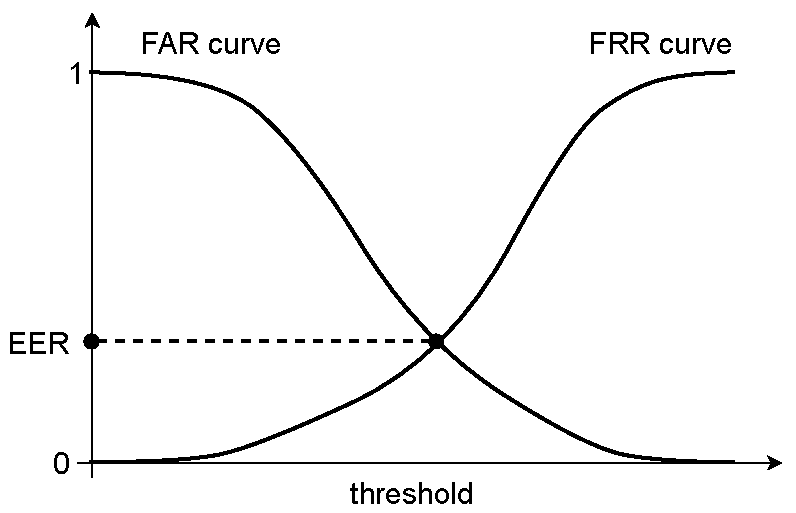
\includegraphics[height=2.1in]{images/EER.pdf}
\caption{The typical curves of the \acs{far} and \acs{frr} error rates, plotted side by side, in relation to the threshold $\tau$ configured for the system. The \acs{eer} is represented by the intersection point of the curves. Source: own elaboration.}
\label{fig:eer}
\end{figure}

Since \acs{far} and \acs{frr} are computed for a given threshold $\tau$, the biometric systems can be calibrated by manually choosing the threshold that best fit the desired needs. However, it represents a trade-off between convenience and security. For example, when security issues are critical (e.g., banking systems), the threshold $\tau$ may be adjusted in a way that the \acs{far} is minimal. However, genuine users may have their access blocked until the system is entirely sure about their profile. On the other side, if $\tau$ is fine-tuned to improve users' convenience, the system can allow access of non-legitimate users.

\subsection{The \icao Standard}

In 1980, the \acf{icao} began a project focused on the standardization of automatic biometric identification of people using machines \citep{icao2003report}. A specific working group was established to determine the most suitable way of ``uniquely encoding a particular physical characteristic of a person into a biometric-identifier that can be machine-verified to confirm the presenter's identity'' \citep{icao2003report}. Initially, three physical attributes were chosen for possible applications: face, fingerprint, and iris. Later, in the ``Berlin resolution'' (2002), the ICAO has chosen the face as the primary globally inter-operable biometric trait for machine-assisted identity confirmation in machine-readable travel documents (MRTDs) \citep{ferrara2012face}. However, the decision also states the possibility of identity confirmation through fingerprint or iris to support the machine-assisted decision.

Following the ICAO guidelines, the \acf{iso}, together with the \acf{iec}, proposed a standard for facial photography to be used in electronic passports. The \icao \citep{iso-iec} standard specifies rules and a record format for encoding, recording, and transmitting facial image information. It also defines a set of environmental conditions, photographic properties, shooting features, and digital image attributes of facial images. For example, a face image may have a uniform background with the absence of shadows in any region of the image to be included in an electronic passport. The complete list of requirements can be seen in Table \ref{tab:icao} and examples of non-compliant images for each requirement are given in Figure \ref{fig:icao}. The \icao standard is also referenced in the ANSI/NIST-ITL 1–2011 standard \citep{nist2011} as one of the standard profiles for face acquisition. In 2019, a new version of the \icao standard was released. The \icaonew provides more detailed information about each requirement evaluation.

\begin{table}[tb]
% \scriptsize
\footnotesize
% \small
\centering
\caption{Description of facial image quality tests performed by \biolab, according to \icao standard.}
\label{tab:icao}
\begin{tabular}{|c|c|}
\hline
\rowcolor[HTML]{9B9B9B} 
\textbf{Req. \#} & \textbf{Test description} \\ \hline
\rowcolor[HTML]{C0C0C0} 
\multicolumn{2}{|c|}{\cellcolor[HTML]{C0C0C0}\textbf{Facial feature extraction tests}} \\ \hline
1 & Eye center location accuracy \\ \hline
2 & Face location accuracy \\ \hline
\rowcolor[HTML]{C0C0C0} 
\multicolumn{2}{|c|}{\cellcolor[HTML]{C0C0C0}\textbf{Geometric tests}} \\ \hline
3 & Eyes distance (min. 90 pixels) \\ \hline
4 & Relative vertical position \\ \hline
5 & Relative horizontal position \\ \hline
6 & Ratio of head width \\ \hline
7 & Ratio of head height \\ \hline
\rowcolor[HTML]{C0C0C0} 
\multicolumn{2}{|c|}{\cellcolor[HTML]{C0C0C0}\textbf{Photographic and pose-specific tests}} \\ \hline
8 & Blurred \\ \hline
9 & Looking away \\ \hline
10 & Ink marked/creased \\ \hline
11 & Unnatural skin tone \\ \hline
12 & Too dark/light \\ \hline
13 & Washed out \\ \hline
14 & Pixelation \\ \hline
15 & Hair across eyes \\ \hline
16 & Eyes closed \\ \hline
17 & Varied Background \\ \hline
18 & Roll/pitch/yaw rotations greater than a predefined thresholds \\ \hline
19 & Flash reflection on skin \\ \hline
20 & Red eyes \\ \hline
21 & Shadows behind head \\ \hline
22 & Shadows across face \\ \hline
23 & Dark tinted lenses \\ \hline
24 & Flash reflection on lenses \\ \hline
25 & Frames too heavy \\ \hline
26 & Frame covering eyes \\ \hline
27 & Hat/cap \\ \hline
28 & Veil over face \\ \hline
29 & Mouth open \\ \hline
30 & Presence of other faces or toys too close to face \\ \hline
\end{tabular}
\end{table}

\begin{figure}[ht]
\centering
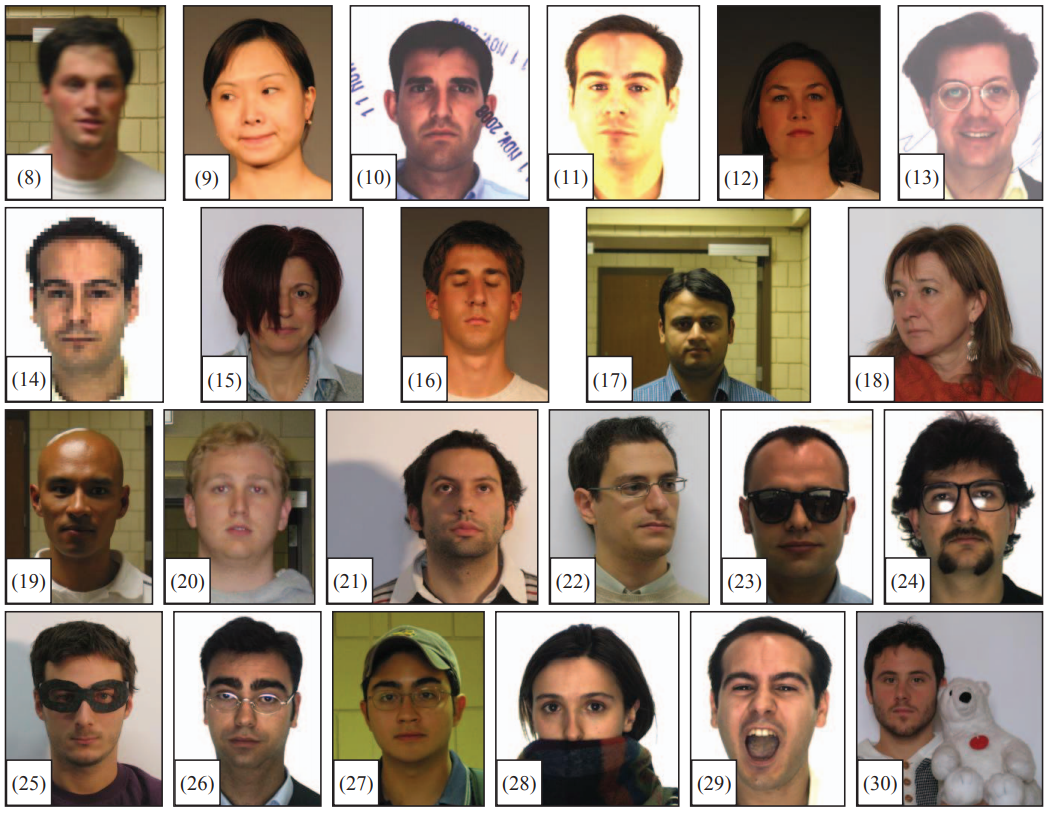
\includegraphics[width=\linewidth]{images/icao.png}
\caption{Examples of non-compliant images for the requirements 8-30 listed in Table \ref{tab:icao}. Source: \cite{maltoni2009biolab}.}
\label{fig:icao}
\end{figure}

\subsection{\fvcongoing} \label{sec:fvcongoing}

The \acf{fvc} is an event organized by four main institutions: \textit{Biometric System Laboratory} (University of Bologna), \textit{Pattern Recognition and Image Processing Laboratory} (Michigan State University), \textit{Biometric Test Center} (San Jose State University), and \textit{Biometric Recognition Group - ATVS} (Universidad Autonoma de Madrid). The main goal of the \acs{fvc} was to benchmark systems that evaluate fingerprint images. Initially, the competitions used to happen biannually (2000, 2002, 2004, and 2006), and such events draw attention from the academic community and the industry related to biometric. Over the years, the \acs{fvc} became a reference in the evaluation of fingerprint systems, allowing research groups, private companies, and even individual developers to compare their methods and follow the state-of-art in fingerprint research.

After 2006, the organizers of \acs{fvc} decided to create the \fvcongoing. It turned the original biannual \acs{fvc} into an ongoing competition, i.e., every participant could register and submit new algorithms in a continuous fashion. Moreover, new competitions regarding fingerprints were added to \fvcongoing, like fingerprint orientation extraction, fingerprint indexing, and minutiae matching.

In 2012, a new benchmark category related to the \icao standard was added to \fvcongoing \citep{ferrara2012face}, called \textit{\acl{ficv}} (\acs{ficv}). The main goal of this benchmark is to evaluate algorithms that assess the compliance of face images to ISO standard. In total, 24 out of 30 requirements are evaluated by the \acs{ficv}: the \citeReq{\eyecenterlocation} and all the photographic and pose-specific tests (8--30) - see \autoref{tab:icao}. Moreover, the \acs{ficv} also evaluates if the image can be converted to a Token Format (see Section 9.2.3 in \citep{iso-iec}) based on the eye positions predicted by a submitted algorithm. In short, an image is considered \textit{tokenizable} (without padding) if:

\begin{itemize}
\item the distance ($E_{Dist}$) between eyes is at least 60 pixels;
\item the rectangular region of size $W \times H$ (with $W=4\cdot E_{Dist}$ and $H=W \cdot 4/3$), determined so that the eyes are horizontally aligned and their center is in position $C_E=(W\cdot1/2,W\cdot3/5)$, is totally enclosed in the original image (see \autoref{fig:icao_token}).
\end{itemize}

\begin{figure}[ht]
    \centering
    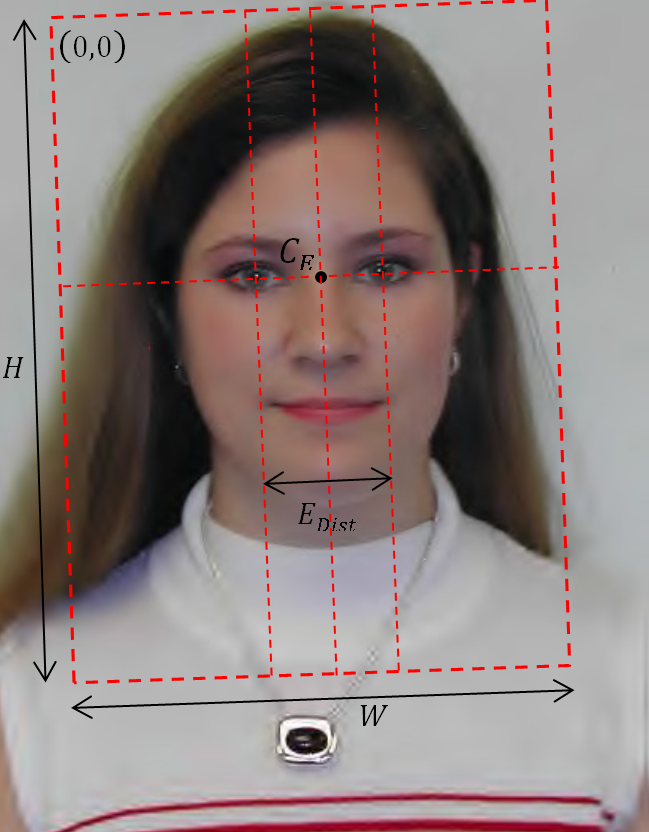
\includegraphics[height=3.0in]{images/icao_tokenizable.png}
    \caption{Geometric characteristics of the token image format. Source: \citep{fvcongoing}.}
    \label{fig:icao_token}
\end{figure}

There are two datasets used to benchmark the algorithms submitted to \acs{ficv} competition: \ficvtest and \ficvofficial. The \ficvtest is a small, but representative dataset (720 images) only used to test the submitted algorithm compliance with the testing protocol (described below). The results computed on this dataset are only visible to the participant and are not considered as official results of the competition. On the other hand, the \ficvofficial contains 4868 images and is private to all participants. Such dataset is detailed in \cite{ferrara2012face}. All the results presented in the literature and in this thesis proposal were computed in the \ficvofficial dataset.

All participants that want to submit an algorithm for evaluation in the \acs{ficv} competition must follow a well-defined protocol. The algorithm must be submitted as a Windows 32 bits (Win32) console application in the format of an executable file. Such executable receives a face image as input and must output the coordinates $(x, y)$ of left-and-right eyes center and a score in the range of $[0, 100]$ to indicate the compliance degree of the input image for each photographic requirement of \autoref{tab:icao}.

Additionally to the submission protocol, the algorithm must still comply with some constraints. For example, the maximum time allowed for the processing of each image is 10 seconds. In case of time violations, the current image evaluation is considered a failure. Also, there is a minimum break of 12 hours between two consecutive submissions by the same participant to the \ficvtest dataset. For the \ficvofficial, this interval is 15 days. However, there are no constraints about memory allocation limit.

Finally, since the requirements \#1 and \#8--30 (see \autoref{tab:icao}) represents different kinds of problems, they are evaluated differently. The \citeReq{\eyecenterlocation} performance is measured by the relative error according to the distances between the expected and the estimated eye positions ($d_{eye}$). This is the same metric introduced by \cite{jesorsky2001robust} and is calculated as follows (\autoref{eq:icao-eyes}):

\begin{equation}
\label{eq:icao-eyes}
d_{eye} = \frac{max(\left\| C_l - \hat{C_l} \right\|, \left\| C_r -\hat{C_r}|\right\|)}{\left\| C_l - C_r \right\|}
\end{equation}

\noindent
where $C_{l/r}$ and $\hat{C_{l/r}}$ represent the ground truth and the positions returned by the algorithm regarding the left and right eyes, respectively. This measure is scale-independent and allows to compare datasets with different image resolutions.

Furthermore, to evaluate the performance of the photographic and pose-specific requirements, the benchmark datasets are divided into 23 different subsets, each related to a specific requirement. Also, each subset contains the same amount of compliant and non-compliant images. Then, for each requirement, the following performance metrics are computed and reported:

\begin{itemize}
\item $EER$: the Equal Error Rate;
\item $FAR_{100}$: the lowest FRR for FAR $\leq$ 1\%;
\item $Zero_{FAR}$: the lowest FRR for FAR=0\%;
\item $Zero_{FRR}$: the lowest FAR for FRR=0\%;
\item $Rejection$: percentage of images where the algorithm did not evaluate the requirement;
\item $Impostor$ and $Genuine$ score distributions;
\item $FAR(\tau) / FRR(\tau)$ curves, where $\tau$ represents the acceptance threshold; and
\item $DET(\tau)$ curve: the Detection Error Tradeoff, which plot the \acl{frr} vs. the \acl{far}.
\end{itemize}

According to \acs{ficv}, the rejections are implicitly included in the computation of metrics in order to discourage the algorithm from rejecting the most uncertain cases and, consequently, improving the performance over the processed images. In these cases, the compliance score is set to 0 in the corresponding requirement of the given image. It follows the best practices of evaluation systems and is also performed in other benchmarks of the \fvcongoing.

In the next chapter, we present a literature analysis related to the current thesis. It focuses on the most relevant published methods for Multitask Learning and the \icao standard, which are the core concepts of the proposed method.
